% 中文图注需要支持中文的LaTeX文档。
\begin{figure*}[t]
\centering
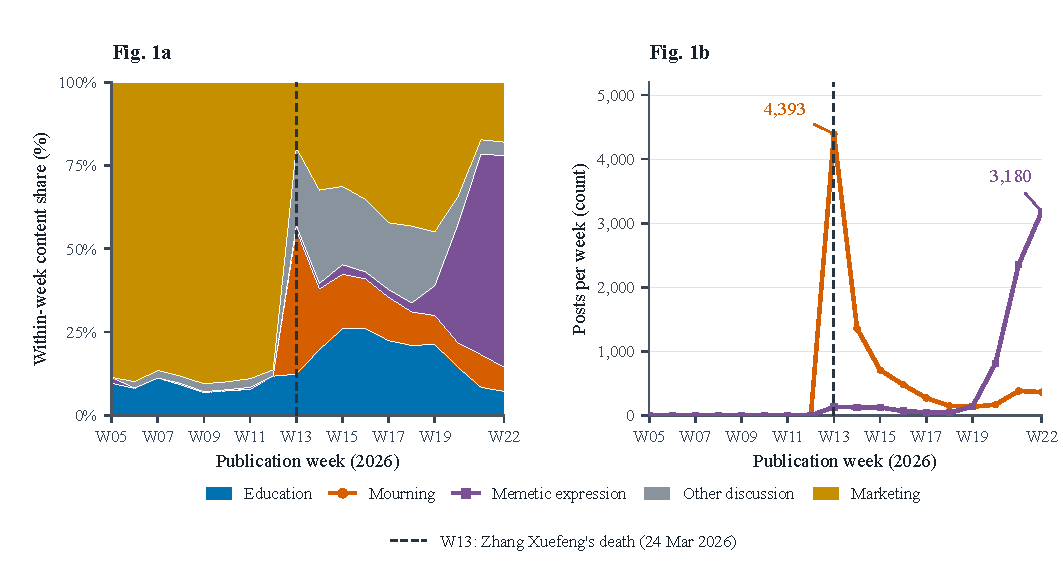
\includegraphics[width=\textwidth]{figure_01_observed_pooled.pdf}
\caption{抖音与小红书合并样本中内容构成及悼念、玩梗表达的周度演化。 图1a展示教育、悼念、玩梗、其他讨论和营销五类内容在各周的构成比例；图1b展示悼念与玩梗帖文的周度数量，关键数字标签标示悼念峰值及末周玩梗数量。横轴为2026年ISO周，范围为W05—W22；竖直虚线标记张雪峰逝世所在周W13，逝世日期为2026年3月24日。颜色区分类别，图1b另用不同点形区分两类表达，相邻周之间直接连线，不进行曲线平滑。原始语料共49,930条，五类分析实际纳入46,602条，未纳入3,315条爬取噪音及13条存疑标签；比例先合并两个平台各类别计数，再以当周五类内容总数为分母计算。数量与比例均来自既有模型辅助编码结果，不设置抽样误差条。}
\label{fig:seed10-1}
\end{figure*}

% 中文图注需要支持中文的LaTeX文档。
\begin{figure*}[t]
\centering
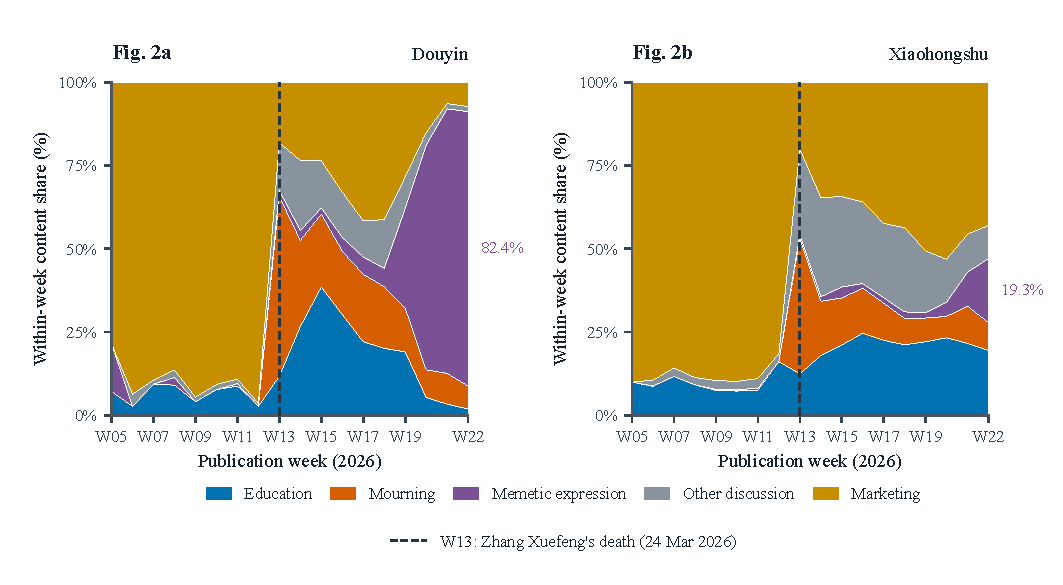
\includegraphics[width=\textwidth]{figure_02_observed_platforms.pdf}
\caption{抖音与小红书五类内容构成的周度比较。 图2a为抖音，图2b为小红书。两面板采用相同的时间轴、0—100\%比例轴与类别配色，颜色依次对应教育、悼念、玩梗、其他讨论和营销；末周标注用于辅助比较玩梗比例。竖直虚线标记张雪峰逝世周W13（2026年3月24日）。横轴为2026年W05—W22，各平台每周五类内容的合计数分别作为该平台当周的比例分母，两个平台的周比例不作简单平均。样本筛选与图1一致，五类合计纳入46,602条，其中抖音15,186条、小红书31,416条。图中反映的是各平台内部的内容构成，面板面积不代表两个平台样本量或流量份额。}
\label{fig:seed10-2}
\end{figure*}

% 中文图注需要支持中文的LaTeX文档。
\begin{figure*}[t]
\centering
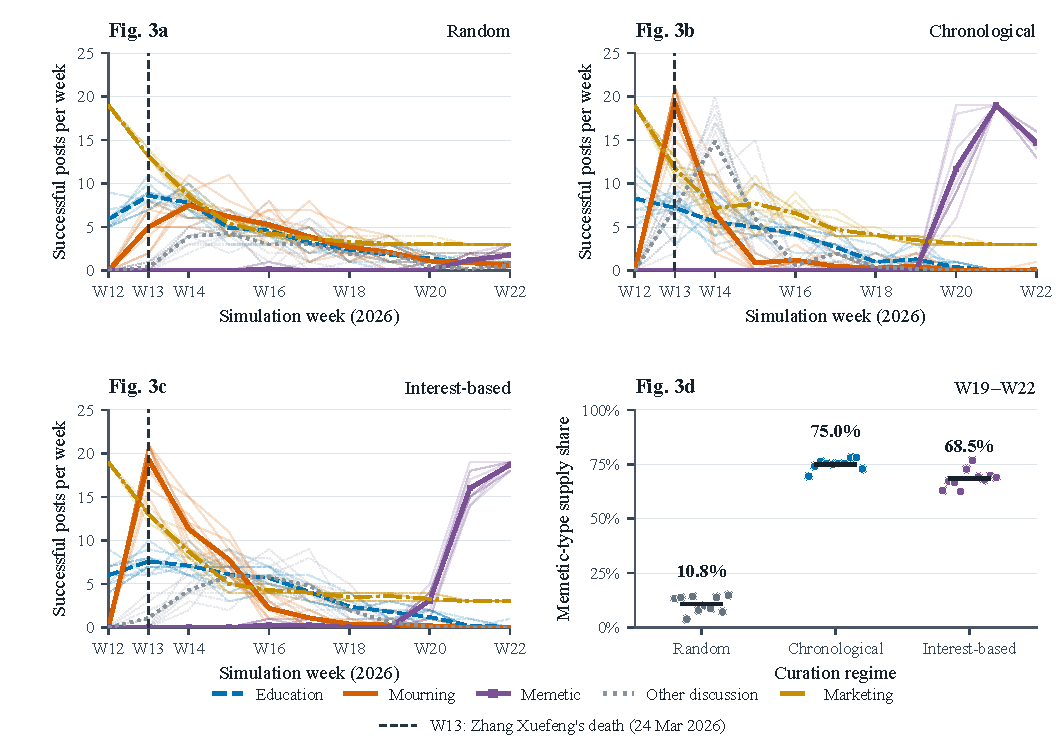
\includegraphics[width=\textwidth]{figure_03_simulated_trajectories.pdf}
\caption{三种策展制度下固定作者类型的供给轨迹及晚期玩梗型供给份额。 图3a—c分别展示随机、时序和兴趣制度下五种固定作者类型在W12—W22的每周成功发帖数量，采用相同的时间轴、数量轴和类别配色；细线为单个种子的轨迹，粗线为10个种子的算术均值。竖直虚线标记张雪峰逝世周W13（2026年3月24日）。图3d展示W19—W22玩梗型作者的供给份额，散点为各次运行，黑色短横线及数字为10次运行的均值，随机、时序和兴趣制度分别为10.8\%、75.0\%和68.5\%。每种制度包含seed 0—9，共30次主运行；份额先在每次运行内以该时期全部智能体成功发帖为分母计算，再跨种子平均。外部输入与历史初始帖不计入作者供给，类型依据固定作者身份而非生成文本的独立语义重分类确定。主分析按本研究已采纳的模型版本等价约定合并原3组与新增7组，分批结果仅作补充稳健性检查；细线和散点反映实际运行差异，不是置信区间。}
\label{fig:seed10-3}
\end{figure*}

% 中文图注需要支持中文的LaTeX文档。
\begin{figure*}[t]
\centering
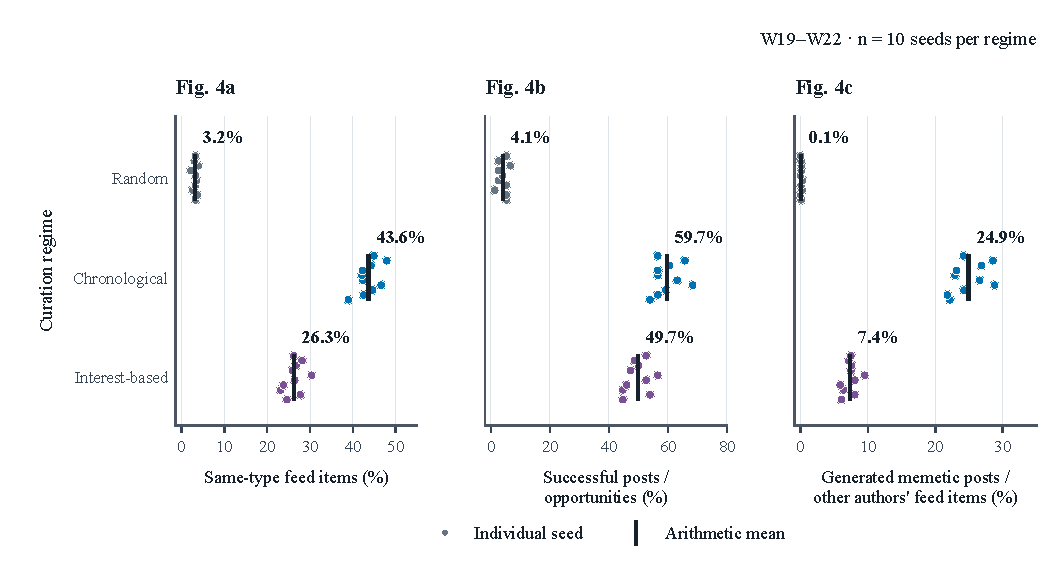
\includegraphics[width=\textwidth]{figure_04_feedback_exposure.pdf}
\caption{三种策展制度下的个人接触、表达参与及生成帖跨群体再展示。 图4a展示W19—W22玩梗型作者个人信息流中的同类内容比例；图4b展示该群体成功发帖数占表达机会的比例；图4c展示玩梗型作者生成帖在其他作者全部信息流展示中的份额。各面板的点为每制度10个种子的实际指标，黑色均值标记及数字为跨种子的算术均值。三项指标均先在每次运行内计算：图4a的分母为玩梗型群体实际获得的760条信息流展示，图4b为19名玩梗型作者在4周内的76次表达机会，图4c为其他作者实际获得的3,240条信息流展示。图4a包含外部帖与生成帖，图4c的分子仅包括来自玩梗型作者的生成帖；生成帖按固定作者类型追踪。随机、时序与兴趣制度的同类接触均值分别为3.2\%、43.6\%和26.3\%，发帖率为4.1\%、59.7\%和49.7\%，生成帖跨群体再展示份额为0.1\%、24.9\%和7.4\%。这些过程指标描述反馈链条中的关联，不单独识别内容回流的净因果贡献。}
\label{fig:seed10-4}
\end{figure*}

% 中文图注需要支持中文的LaTeX文档。
\begin{figure*}[t]
\centering
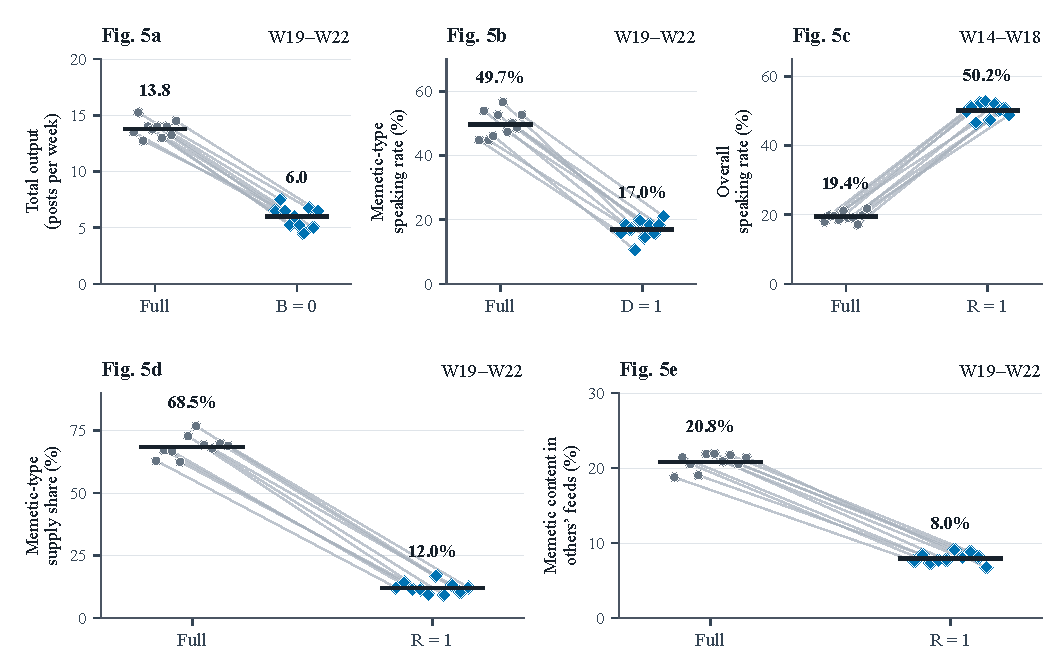
\includegraphics[width=\textwidth]{figure_05_bdr_ablation.pdf}
\caption{表达组件干预对参与、供给及可见位置的影响。（a）比较完整模型与B=0条件下W19—W22的平均每周总供给；（b）比较完整模型与D=1条件下同期玩梗型作者的发言率；（c）比较完整模型与R=1条件下W14—W18全体作者的发言率；（d）、（e）分别比较R=1条件下W19—W22玩梗型作者的供给份额，以及其他作者信息流中玩梗内容的比例。B=0将常态表达基线置零，D=1将意见气候响应固定为1，R=1将事件注意力权重固定为1。各比较均在兴趣策展制度下进行，人口构成、外部输入和行动安排保持一致，每种条件包含10个种子（seed 0—9），完整模型复用对应的10次主运行。散点表示各次运行，灰线连接同一种子的完整模型与干预条件，黑色短横线及数字表示跨种子均值。发言率以相应群体的表达机会为分母，供给份额以同期全部智能体成功发帖为分母；图5e的分子同时包含外部帖与生成帖，分母为其他作者实际获得的信息流展示。}
\label{fig:seed10-5}
\end{figure*}
